\section{课题的提出及背景}
\subsection{国内外车门的发展现状}
德国、奥地利和日本的铁路工业是世界的佼佼者,尤其是日本的铁路新干线开创了日本铁路产业的里程碑,也为其他国家铁路事业的发展树立了榜样。在车门的研究方面日本也有实质性的突破,尤其表现在自动关门机的开发上。他们在设计通勤电动客车时,车门没有设台阶,以便旅客能平稳流动以及安全、迅速上下车,具有缩短停车时间的显著功能。

为了缓和客流高峰、缩短上下车时间,从209系、E217系以后的“新系列车辆”起,JR东日本客运公司就在市郊型电力客车一侧设置了4个车门,并将其规定为通勤电动客车的车门设置标准。为了贯彻该自动关门机要求的“高可靠性、操纵力易于控制、减少修理”的新理念,JR东日客公司于1992年首次开发了电气式自动关门机构,并安装于901系列编组车上在京摈东北根岸线上试用。
\begin{figure}[hp]
    \centering
    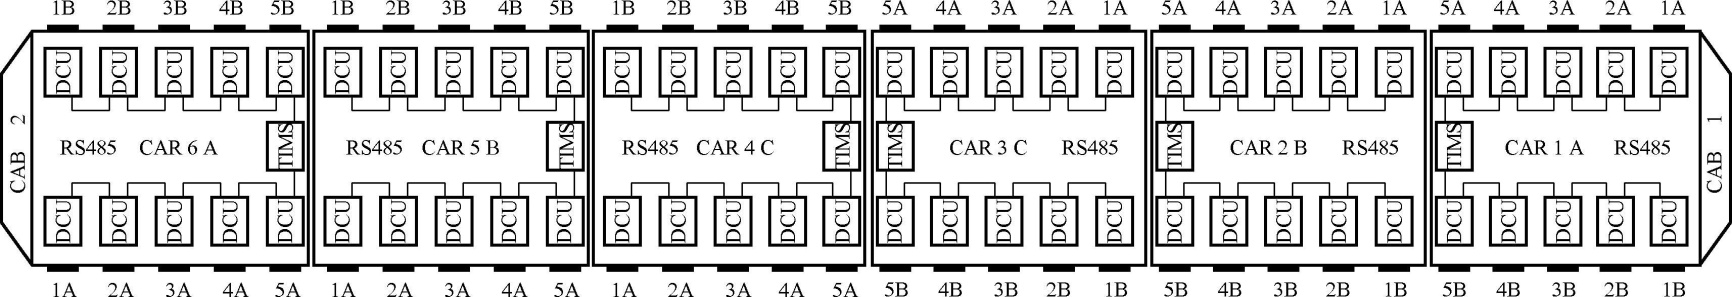
\includegraphics[width=0.8\textwidth]{figures/train.png}
    \caption{轨道车辆车门分布简图}
    \label{fig:train_railways}
\end{figure}


